\PassOptionsToPackage{bookmarks={true}}{hyperref}
\pdfminorversion=4
\documentclass[mathserif,xcolor={dvipsnames,table}]{beamer}
\mode<presentation>{\usetheme{Warsaw}\usecolortheme{crane}}
\usepackage{centernot}
\usepackage{upgreek}
\usepackage{graphicx}
\usepackage{geometry}
\usepackage{transparent}
\usepackage{tikz}
\usetikzlibrary{shadows}
\usepackage[utf8]{inputenc}
\usepackage[english]{babel}
\usepackage[T1]{fontenc}
\usepackage{lmodern}
\usepackage[babel=true]{microtype}
\usepackage{amsmath}
\beamertemplatenavigationsymbolsempty

\title{\textbf{Big-$\boldsymbol{\mathcal{O}}$ Ain't What it Used to Be}}
\date{}
\author{CS4803UWS at the\\
Georgia Institute of Technology
}

\begin{document}

{
\setbeamertemplate{background canvas}{%
\includegraphics[width=\paperwidth,height=\paperheight]{images/gt2.jpeg}
}%
\begin{frame}[plain]
\textcolor{white}{
\transparent{0.5}%
\colorbox{black}{\textbf{Big-$\boldsymbol{\mathcal{O}}$ Ain't What it Used to Be}}
}
\vspace{2.7in}
\\
\hfill\includegraphics[scale=.25]{images/cc-logo.pdf}

\includegraphics[scale=.25]{images/cc-new.pdf}

\includegraphics[scale=.25]{images/cc-share.pdf}
\textcolor{white}{
\\
\hfill \tiny{CC3.0 share-alike attribution}\\
}
\textcolor{white}{
\hfill \scriptsize{copyright \copyright\ 2013}\\
}
\end{frame}
}

\begin{frame}{Asymptotic notation review I}
Asymptotic analysis gives us a means of speaking of arbitrarily large growth,
independently of arbitrarily (but finitely) large costs not associated with
problem size.
\scriptsize{
\begin{center}
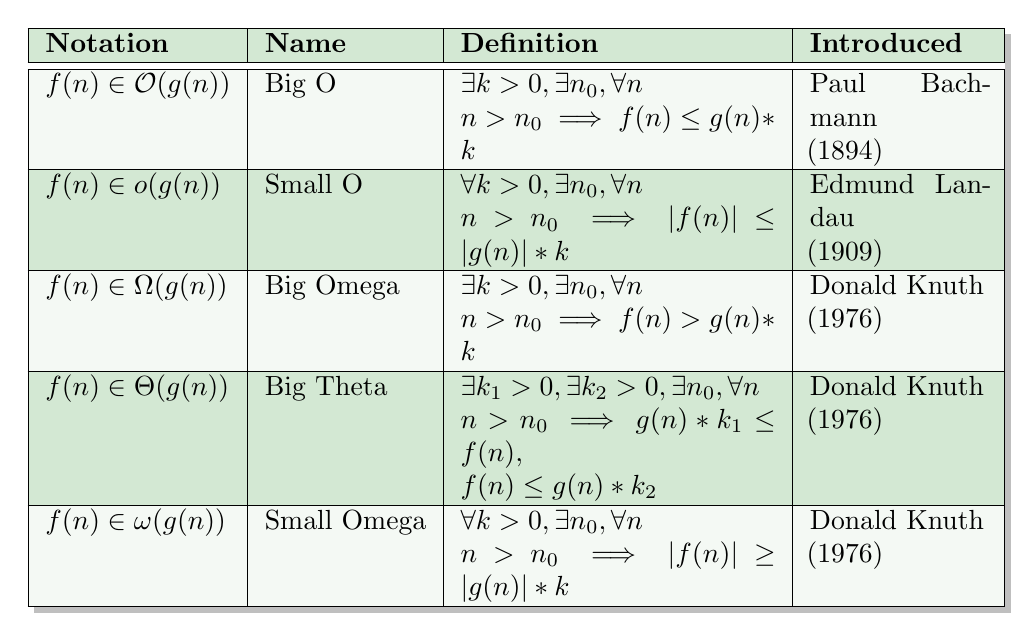
\begin{tikzpicture}
\node[drop shadow,fill=white,inner sep=0pt]
{\rowcolors{1}{ForestGreen!20}{ForestGreen!5}
\begin{tabular}{|l|l|p{4cm}|p{2.25cm}|}
\hline
\textbf{Notation} & \textbf{Name} & \textbf{Definition} & \textbf{Introduced} \\
\hline\hline
$f(n) \in \mathcal{O}(g(n))$ & Big O & $\exists k>0,\exists n_0,\forall n$
\newline
$n>n_0 \implies f(n) \le g(n)*k$ & Paul Bachmann\newline (1894) \\
\hline
$f(n) \in o(g(n))$ & Small O & $\forall k>0,\exists n_0,\forall n$
\newline
$n>n_0 \implies |f(n)| \le |g(n)|*k$ & Edmund Landau\newline (1909) \\
\hline
$f(n) \in \Omega(g(n))$ & Big Omega & $\exists k>0,\exists n_0,\forall n$
\newline
$n>n_0 \implies f(n) > g(n)*k$ & Donald Knuth\newline (1976) \\
\hline
$f(n) \in \Theta(g(n))$ & Big Theta & $\exists k_1>0,\exists k_2>0,\exists n_0,\forall n$
\newline
$n>n_0 \implies g(n)*k_1 \le f(n),
\newline
f(n) \le g(n)*k_2$ & Donald Knuth\newline (1976) \\
\hline
$f(n) \in \omega(g(n))$ &Small Omega& $\forall k>0,\exists n_0,\forall n$
\newline
$n>n_0 \implies |f(n)| \ge |g(n)|*k$ & Donald Knuth\newline(1976) \\
\hline
\end{tabular}%
};
\end{tikzpicture}
\end{center}
\vfill
Advances in (finite) computing technology can only reduce these
ignored costs. Wrap the earth with your register file, and still there will be
numbers so large that their addition is $\Theta(n)$.
}
\end{frame}

\begin{frame}{Asymptotic notation review II}
\scriptsize{
\begin{center}
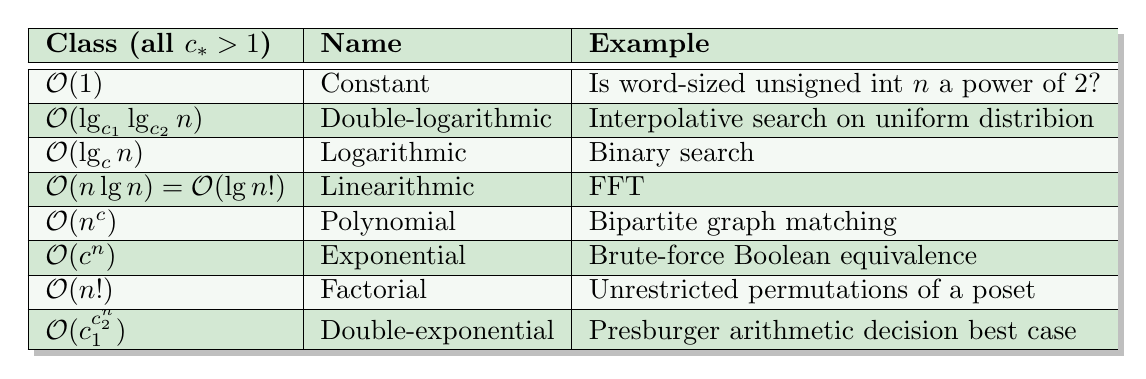
\begin{tikzpicture}
\node[drop shadow,fill=white,inner sep=0pt]
{\rowcolors{1}{ForestGreen!20}{ForestGreen!5}
\begin{tabular}{|l|l|l}
\hline
\textbf{Class (all $c_*>1$)} & \textbf{Name} & \textbf{Example} \\
\hline\hline
$\mathcal{O}(1)$ & Constant & Is word-sized unsigned int $n$ a power of 2?\\
\hline
$\mathcal{O}(\lg_{c_1}\lg_{c_2} n)$ & Double-logarithmic & Interpolative search on uniform distribion\\
\hline
$\mathcal{O}(\lg_c n)$ & Logarithmic & Binary search\\
\hline
$\mathcal{O}(n\lg n) = \mathcal{O}(\lg n!)$ & Linearithmic & FFT\\
\hline
$\mathcal{O}(n^{c})$ & Polynomial & Bipartite graph matching\\
\hline
$\mathcal{O}(c^{n})$ & Exponential & Brute-force Boolean equivalence \\
\hline
$\mathcal{O}(n!)$ & Factorial & Unrestricted permutations of a poset\\
\hline
$\mathcal{O}(c^{c^{n}_2}_1)$ & Double-exponential & Presburger arithmetic decision best case\\
\hline
\end{tabular}%
};
\end{tikzpicture}
\end{center}
\vfill
Speaking of still faster growth rates\footnote{\scriptsize{Check out ``fast-growing hierarchies'' and the L\"ob–Wainer hierarchy.}} (hyper-exponential, $\mathcal{A}(n)$)
 is mostly zoology\footnote{\scriptsize{Forgive the pun on busy beavers.}}.
}
\end{frame}

\begin{frame}{It's the constants, stupid}
Algorithmic choices can dominate performance, especially at scale. By the
definition of Big O, it should also be obvious that an asymptotically superior
algorithm can be slower for small inputs\footnote{We will see that small inputs can be surprisingly large.}.\\
\vfill
That said, no one's going to think implementing a routing table with a linked list is a good idea.\\
\vfill
Furthermore, asymptotic analysis speaks of performance as problem size grows.
It doesn't speak of real-time. It doesn't speak of bounded memories.
We rarely speak of piecewise asymptotics.
\vfill
But, by all means, do ensure you're not doing linear searches on sorted data etc.
\end{frame}

\begin{frame}{What's hiding behind $\mathcal{O}$?}
Naive $nxn$ matrix multiplication is $\Theta(n^{3})$.
\vfill
\begin{equation}
C = AB \implies C_{ij} = \sum\limits_{m=1}^{k} A_{im}B_{mj}
\end{equation}
\vfill
Counting the explicit additions and multiplications, there are
precisely $2n^{3}$ operations.
\end{frame}


\begin{frame}{Fused multiply-add}
\end{frame}

%In terms of pure growth, we have $ijk$, so we can set
%\begin{equation}
%n=\frac{i}{3} + \frac{j}{3} + \frac{k}{3}
%\end{equation}
%and this is a very accurate analysis.
%Do you see $n$?\\
%\vfill
%I see $k$ additions of $k$ multiplications, done $i * j$ times. So $n$ is the
%average of our three sizes. But really, $k$ contributes twice as much as either
%$i$ or $j$. So
%\begin{equation}
%n = \frac{k}{2} + \frac{i}{4} + \frac{j}{4}
%\end{equation}
%
%naively, a bit at a time on $b$-bit inputs, I see $ijk\Theta(b) + ijk\mathcal{O}(b^{2})
%\implies ijk\mathcal{O}(b^{2})$. Fix $b$. I see $ijkb + ijkb^{2}$. What, we can add
%$b$-bit words in a single operation? I see $ijk + ijkb$
%\footnote{\tiny{Note that whatever $b$ we pick, so long as we pick a finite $b$, the
%asymptotic analysis holds---whether $b$ or $b^{2}$, it's just a constant factor
%as our problem grows. Accurately multiplying matrices of fixed size, but having arbitrarily
%large elements, is a different analysis.}}
%. Ho ho, we have a hardware
%multiplier? $ijk + ijk$ it is!

\begin{frame}{Recommended reading}
\tiny{
\begin{itemize}
\item Goto et al. ``Anatomy of High-Performance Matrix Multiplication'' (2008).
\item Kalyanasundaram et al. ``Improved Simulation of NTMs'' (2011).
\item Fran\c{c}ois Le Gall. ``Faster Algorithms for Rectangular Matrix Multiplication'' (2012).
\item Eric Quinnell. ``Floating-Point Fused Multiply-Add Architectures'' (2007).
\end{itemize}
}
\end{frame}

%\begin{frame}{Hack on!}
%\end{frame}

\end{document}
